\documentclass[journal,12pt,twocolumn]{IEEEtran}
%

\usepackage{setspace}
\usepackage{gensymb}
\singlespacing

\usepackage{amsmath}
\usepackage{amsthm}
\usepackage{txfonts}
\usepackage{cite}
\usepackage{enumitem}
\usepackage{mathtools}
\usepackage{hyperref}
\usepackage{listings}
    \usepackage{color}                                            %%
    \usepackage{array}                                            %%
    \usepackage{longtable}                                        %%
    \usepackage{calc}                                             %%
    \usepackage{multirow}                                         %%
    \usepackage{hhline}                                           %%
    \usepackage{ifthen}                                           %%
  %optionally (for landscape tables embedded in another document): %%
    \usepackage{lscape}     
\usepackage{multicol}
\usepackage{chngcntr}
\renewcommand\thesection{\arabic{section}}
\renewcommand\thesubsection{\thesection.\arabic{subsection}}
\renewcommand\thesubsubsection{\thesubsection.\arabic{subsubsection}}

% correct bad hyphenation here
\hyphenation{op-tical net-works semi-conduc-tor}
\def\inputGnumericTable{}                                 %%

\lstset{
%language=C,
frame=single, 
breaklines=true,
columns=fullflexible
}

\begin{document}
%


\newtheorem{theorem}{Theorem}[section]
\newtheorem{problem}{Problem}
\newtheorem{proposition}{Proposition}[section]
\newtheorem{lemma}{Lemma}[section]
\newtheorem{corollary}[theorem]{Corollary}
\newtheorem{example}{Example}[section]
\newtheorem{definition}[problem]{Definition}
\newcommand{\BEQA}{\begin{eqnarray}}
\newcommand{\EEQA}{\end{eqnarray}}
\newcommand{\define}{\stackrel{\triangle}{=}}
\bibliographystyle{IEEEtran}
\providecommand{\mbf}{\mathbf}
\providecommand{\pr}[1]{\ensuremath{\Pr\left(#1\right)}}
\providecommand{\qfunc}[1]{\ensuremath{Q\left(#1\right)}}
\providecommand{\sbrak}[1]{\ensuremath{{}\left[#1\right]}}
\providecommand{\lsbrak}[1]{\ensuremath{{}\left[#1\right.}}
\providecommand{\rsbrak}[1]{\ensuremath{{}\left.#1\right]}}
\providecommand{\brak}[1]{\ensuremath{\left(#1\right)}}
\providecommand{\lbrak}[1]{\ensuremath{\left(#1\right.}}
\providecommand{\rbrak}[1]{\ensuremath{\left.#1\right)}}
\providecommand{\cbrak}[1]{\ensuremath{\left\{#1\right\}}}
\providecommand{\lcbrak}[1]{\ensuremath{\left\{#1\right.}}
\providecommand{\rcbrak}[1]{\ensuremath{\left.#1\right\}}}
\theoremstyle{remark}
\newtheorem{rem}{Remark}
\newcommand{\sgn}{\mathop{\mathrm{sgn}}}
\providecommand{\abs}[1]{\lvert#1\rvert}
\providecommand{\res}[1]{\Res\displaylimits_{#1}} 
\providecommand{\norm}[1]{\lVert#1\rVert}
\providecommand{\mtx}[1]{\mathbf{#1}}
% \providecommand{\mean}[1]{E\left[ #1 \right]}
\providecommand{\fourier}{\overset{\mathcal{F}}{ \rightleftharpoons}}
\providecommand{\system}{\overset{\mathcal{H}}{ \longleftrightarrow}}
\newcommand{\solution}{\noindent \textbf{Solution: }}
\newcommand{\cosec}{\,\text{cosec}\,}
\providecommand{\dec}[2]{\ensuremath{\overset{#1}{\underset{#2}{\gtrless}}}}
\newcommand{\myvec}[1]{\ensuremath{\begin{pmatrix}#1\end{pmatrix}}}
\newcommand{\cmyvec}[1]{\ensuremath{\begin{pmatrix*}[c]#1\end{pmatrix*}}}
\newcommand{\mydet}[1]{\ensuremath{\begin{vmatrix}#1\end{vmatrix}}}
\newcommand{\proj}[2]{\textbf{proj}_{\vec{#1}}\vec{#2}}
\newcommand{\RNum}[1]{\uppercase\expandafter{\romannumeral #1\relax}}
\let\StandardTheFigure\thefigure
\let\vec\mathbf
\title{
\LARGE SM5083\\
    \LARGE Assignment 1 \\[0.5em]
    
    \large Ravi Kumar\par
    \large   SM21MTECH12010  \par
}
\maketitle
\renewcommand{\thefigure}{\theenumi}
\renewcommand{\thetable}{\theenumi}
\section{ chapter \RNum{2}  example \RNum{2} Q22(i) }
\textbf{Find the conditions that the four points}\\
\vspace{0.1cm}

\myvec{x1\\y1}, \myvec{x2\\y2},
\myvec{x3\\y3}, \myvec{x4\\y4}\\

\vspace{0.1cm}
\textbf{ may be the vertices of a square.}

\solution
\begin{align}
    ~\text{Given}~\\ \vec{A} = \myvec{x1\\y1}, \vec{B} = \myvec{x2\\y2}, \vec{C} = \myvec{x3\\y3}, \vec{D} = \myvec{x4\\y4}
\end{align}

Condition for the given four points be the vertices of a square are ;-\\
1) If distance between all the four sides are equal and\\
2) distance between two diagonals are equal.
\vspace{0.2cm}
Now If we have two vectors, say,
\begin{align}
    \vec{U} = \myvec{x1\\y1}\ ~\text{and}~
    \vec{V} = \myvec{x2\\y2} 
\end{align}
then distance can be calculated using norm of a vector, i.e., 
\begin{align}
\label{Equation 3}
\norm{ \vec{U} - \vec{V}} = \vec{\sqrt{(u1-v1)^2+(u2-v2)^2}}
\end{align}
Here, From equations  
    \eqref{Equation 3}
\begin{align}
\label{Equation 4}
\norm{ \vec{A} - \vec{B}} =\vec{\sqrt{(x2-x1)^2+(y2-y1)^2}}\\
\label{Equation 5}
\norm{ \vec{B} - \vec{C}} =\vec{\sqrt{(x3-x2)^2+(y3-y2)^2}}\\
\label{Equation 6}
\norm{ \vec{C} - \vec{D}} =\vec{\sqrt{(x4-x3)^2+(y4-y3)^2}}\\
\label{Equation 7}
\norm{ \vec{D} - \vec{A}} =\vec{\sqrt{(x1-x4)^2+(y1-y4)^2}}
\end{align}
and then calculate distance of diagonal using 
\begin{align}
\label{Equation 7}
\vec{diagonal}=\vec{\sqrt{2}* side length}
\end{align}
Now from equations 
\eqref{Equation 4}, \eqref{Equation 5}, \eqref{Equation 6} and \eqref{Equation 7}\\
if,
\begin{align}
\label{Equation 8}
\norm{ \vec{A} - \vec{B}}=\norm{ \vec{B} - \vec{C}}=\norm{ \vec{C} - \vec{D}}=\norm{ \vec{D} - \vec{A}}
\end{align}
And from equation 
\eqref{Equation 7}, calculate diagonal of square\\
if,
\begin{align}
\label{Equation 9}
\vec{diagonal1} = \vec{diagonal2}
\end{align}
Now from equation 
\eqref{Equation 8} and \eqref{Equation 9}\\
if both equation satisfy\\
\textbf{Then, we can say that the given point are the vertices of a square.}
\\
\newline Python code at:
\begin{lstlisting}
https://github.com/ravi12010/SM5083_Assignment1/blob/main/Assignment_1.ipynb
\end{lstlisting}
% https://github.com/ravi12010/SM5083_Assignment1/blob/main/Assignment_1.ipynb{Python Code}
\begin{figure}[!ht]
	\centering
	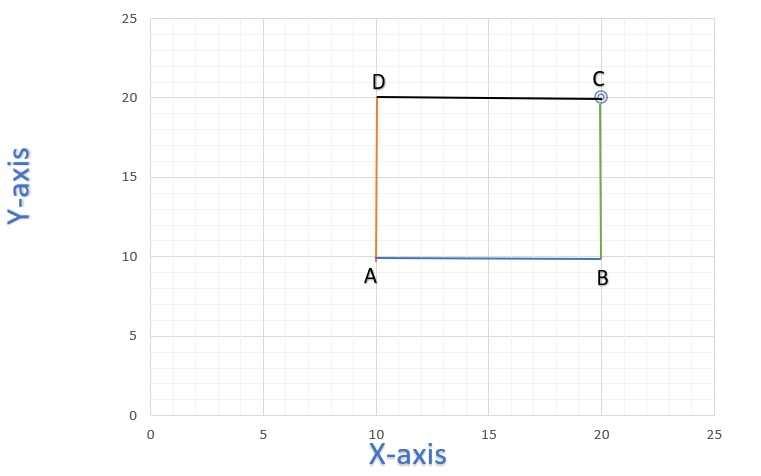
\includegraphics[width=\columnwidth]{square.jpg}
	\caption{The given points form a square}
	\label{fig:Square}
\end{figure}
\end{document}